% ============================================================
%  DISCOVERY CURRICULUM — Journey 4, Module 6
%  "Curved Spaces and General Relativity"
%  Compile with: pdflatex J4_M6.tex  (run twice)
% ============================================================
\documentclass[12pt,a4paper]{article}
\usepackage[a4paper,top=2.5cm,bottom=2.5cm,left=2.8cm,right=2.8cm,headheight=15pt]{geometry}
\usepackage{amsmath,amssymb,amsthm}
\usepackage{xcolor}
\usepackage{mdframed}
\usepackage{enumitem}
\usepackage{tikz}
\usetikzlibrary{arrows.meta,calc}
\usepackage{pgfplots}
\pgfplotsset{compat=1.18}
\usepackage{booktabs}
\usepackage{fancyhdr}
\usepackage{titlesec}
\usepackage{parskip}
\usepackage{hyperref}
\hypersetup{colorlinks=true,linkcolor=NavyBlue,urlcolor=NavyBlue}

\definecolor{NavyBlue}{HTML}{1A3A5C}
\definecolor{MidBlue}{HTML}{2E6DA4}
\definecolor{Gold}{HTML}{C8922A}
\definecolor{LightBlue}{HTML}{EBF2FA}
\definecolor{LightGold}{HTML}{FDF4E3}
\definecolor{DarkGrey}{HTML}{3A3A3A}
\definecolor{BoxGreen}{HTML}{E8F5E9}
\definecolor{SidebarGrey}{HTML}{F5F5F5}

\titleformat{\section}{\Large\bfseries\color{NavyBlue}}{}{0em}{}[{\color{MidBlue}\vspace{2pt}\rule{\linewidth}{1.5pt}}]
\titleformat{\subsection}{\large\bfseries\color{MidBlue}}{}{0em}{}

\pagestyle{fancy}\fancyhf{}
\fancyhead[L]{\small\color{DarkGrey}\textit{Discovery Curriculum}}
\fancyhead[R]{\small\color{DarkGrey}\textit{Journey 4 $\cdot$ Module 6}}
\fancyfoot[C]{\small\color{MidBlue}\thepage}
\renewcommand{\headrulewidth}{0.4pt}

\newmdenv[backgroundcolor=NavyBlue!7,linecolor=NavyBlue,linewidth=2pt,leftline=true,rightline=false,topline=false,bottomline=false,innerleftmargin=14pt,innerrightmargin=10pt,innertopmargin=10pt,innerbottommargin=10pt,skipabove=14pt,skipbelow=10pt]{puzzlebox}
\newmdenv[backgroundcolor=LightGold,linecolor=Gold,linewidth=2pt,leftline=true,rightline=false,topline=false,bottomline=false,innerleftmargin=14pt,innerrightmargin=10pt,innertopmargin=10pt,innerbottommargin=10pt,skipabove=14pt,skipbelow=10pt]{discoverybox}
\newmdenv[backgroundcolor=LightBlue,linecolor=MidBlue,linewidth=1.5pt,roundcorner=4pt,innerleftmargin=14pt,innerrightmargin=10pt,innertopmargin=10pt,innerbottommargin=10pt,skipabove=14pt,skipbelow=10pt]{namebox}
\newmdenv[backgroundcolor=BoxGreen,linecolor=DarkGrey!35,linewidth=1pt,roundcorner=4pt,innerleftmargin=14pt,innerrightmargin=10pt,innertopmargin=10pt,innerbottommargin=10pt,skipabove=14pt,skipbelow=10pt]{reflectionbox}
\newmdenv[backgroundcolor=SidebarGrey,linecolor=Gold,linewidth=1.2pt,leftline=true,rightline=false,topline=false,bottomline=false,innerleftmargin=12pt,innerrightmargin=10pt,innertopmargin=7pt,innerbottommargin=7pt,skipabove=10pt,skipbelow=10pt]{thought}

\newcounter{problem}
\newenvironment{problem}[1][]{\refstepcounter{problem}\par\vspace{6pt}\noindent\textbf{\color{MidBlue}Problem \theproblem}\ifx&#1&\else\ \textit{(#1)}\fi\textbf{.}\enskip}{\par\vspace{4pt}}
\newcounter{deepproblem}
\newenvironment{deepproblem}[1][]{\refstepcounter{deepproblem}\par\vspace{6pt}\noindent\textbf{\color{NavyBlue}$\bigstar$\ Deep Problem \thedeepproblem}\ifx&#1&\else\ \textit{(#1)}\fi\textbf{.}\enskip}{\par\vspace{4pt}}

\begin{document}

\thispagestyle{empty}
\begin{center}
{\small\color{MidBlue}\textbf{DISCOVERY CURRICULUM}\quad$\cdot$\quad\textbf{JOURNEY 4: FIELDS AND SPACE}}
\vspace{0.6cm}

{\color{NavyBlue}\rule{\linewidth}{2pt}}\vspace{0.5cm}

{\Huge\bfseries\color{NavyBlue}Module 6}\\[0.3cm]
{\LARGE\bfseries\color{MidBlue}Curved Spaces and General Relativity}\\[0.4cm]
{\color{Gold}\rule{0.4\linewidth}{1.2pt}}\\[0.4cm]
{\large\itshape\color{DarkGrey}
Gravity is not a force. It is the curvature of spacetime.\\[0.15cm]
Matter tells spacetime how to curve;\\[0.15cm]
spacetime tells matter how to move.}\\[0.2cm]
{\footnotesize\color{DarkGrey}--- John Archibald Wheeler}

\vspace{0.9cm}
\begin{tabular}{rl}
\color{DarkGrey}\textbf{Journey}           & Journey 4 --- Fields and Space \\[4pt]
\color{DarkGrey}\textbf{Module}            & 6 of 6 \textit{(final module of Journey 4)} \\[4pt]
\color{DarkGrey}\textbf{Prerequisites}     & J4 Modules 1--5; J3 Modules 3--4 \\[4pt]
\color{DarkGrey}\textbf{You will discover} & Riemannian geometry, metric tensor, curvature, geodesics, Einstein field equations \\[4pt]
\color{DarkGrey}\textbf{Format}            & 7 problems $+$ 3 deep problems $\approx$ 14 pages \\
\end{tabular}
\vspace{1cm}

{\color{NavyBlue}\rule{\linewidth}{2pt}}
\end{center}

\vspace{0.5cm}
\noindent\textbf{Gauss's remarkable theorem.}
In 1827, Gauss proved that the curvature of a surface --- whether it bends like a sphere or saddles like a mountain pass --- can be measured entirely from within the surface, without reference to the ambient space. An ant on a sphere can detect the curvature by measuring the sum of angles in a triangle, or the circumference of a circle. The ant never needs to step off the surface and look from outside. Riemann (1854) extended this to spaces of any dimension, founding the subject of Riemannian geometry. Einstein (1915) realised that spacetime is a four-dimensional Riemannian (actually pseudo-Riemannian) manifold, and that gravity is its curvature. This is general relativity.

\newpage

\section{Part 1 \texorpdfstring{---}{--} The Puzzle}

\begin{puzzlebox}
\textbf{The Opening Puzzle: Parallel transport and curvature.}

Take a tangent vector at the North Pole, pointing south toward Kenya. Transport it along the prime meridian to the equator, always keeping it parallel to itself (tangent to the meridian). At the equator, rotate $90^\circ$ east (still along the equator, parallel transporting). At $90^\circ$E longitude on the equator, transport back to the North Pole along that meridian.

\medskip
\textbf{Question 1.} What direction does your vector point when it returns to the North Pole? Has it rotated? By how much?

\textbf{Question 2.} The rotation angle equals the \emph{solid angle} subtended by the enclosed triangle. Compute it as a fraction of the total solid angle of the sphere.

\textbf{Question 3.} On a flat surface (Euclidean plane), a vector parallel-transported around any closed loop returns to its original direction. The rotation on a curved surface is a measure of curvature. Can you quantify this?

\textbf{Question 4.} The surface of the Earth is positively curved (a sphere). Describe what negatively curved space would look like locally: what happens to triangles, parallel lines, and circles?
\end{puzzlebox}

\section{Part 2 \texorpdfstring{---}{--} Exploration}

\subsection{Step 1: The metric tensor}

\begin{problem}
\label{prob:metric}
The fundamental object of Riemannian geometry is the \textbf{metric tensor} $g_{ij}$, which gives the squared distance between nearby points:
$ds^2 = g_{ij}\,dq^i\,dq^j$ (summing over repeated indices).
\begin{enumerate}[label=(\alph*),topsep=2pt]
  \item In flat $\mathbb{R}^3$ (Cartesian): $ds^2=dx^2+dy^2+dz^2$. Write the metric tensor as a matrix.
  \item In spherical coordinates $(r,\theta,\phi)$: $ds^2=dr^2+r^2d\theta^2+r^2\sin^2\!\theta\,d\phi^2$. Write the metric tensor. (The off-diagonal entries are zero: why are spherical coordinates orthogonal?)
  \item On the unit sphere $S^2$ ($r=1$): $ds^2=d\theta^2+\sin^2\!\theta\,d\phi^2$. Compute the circumference of a circle of co-latitude $\theta_0$ (latitude measured from north pole). Compute the ratio circumference/radius (where radius is measured along the sphere). Show it is less than $2\pi$, consistent with positive curvature.
  \item The metric determines angles and areas. The area element on $S^2$ is $dA = \sqrt{\det g}\,d\theta\,d\phi = \sin\theta\,d\theta\,d\phi$. Compute the total area of $S^2$.
  \item The \textbf{Minkowski metric} of special relativity: $ds^2 = -c^2dt^2+dx^2+dy^2+dz^2$ (signature $-+++$). The metric tensor is $g_{\mu\nu}=\text{diag}(-1,1,1,1)$. A spacetime interval with $ds^2<0$ is \textbf{timelike} (inside the light cone); $ds^2>0$ is \textbf{spacelike}; $ds^2=0$ is \textbf{lightlike}. Interpret physically.
\end{enumerate}
\end{problem}

\subsection{Step 2: Christoffel symbols and geodesics}

\begin{problem}
\label{prob:geodesics}
The \textbf{Christoffel symbols} $\Gamma^k_{ij}$ are defined by
$\Gamma^k_{ij} = \frac{1}{2}g^{k\ell}\left(\partial_i g_{j\ell}+\partial_j g_{i\ell}-\partial_\ell g_{ij}\right)$
where $g^{k\ell}$ is the inverse metric. They encode how the basis vectors change from point to point.
\begin{enumerate}[label=(\alph*),topsep=2pt]
  \item Compute the non-zero Christoffel symbols for $S^2$ with metric $g_{\theta\theta}=1$, $g_{\phi\phi}=\sin^2\theta$. You should find $\Gamma^\theta_{\phi\phi}=-\sin\theta\cos\theta$ and $\Gamma^\phi_{\theta\phi}=\Gamma^\phi_{\phi\theta}=\cot\theta$.
  \item The \textbf{geodesic equation} is $\ddot q^k + \Gamma^k_{ij}\dot q^i\dot q^j = 0$ (from Euler-Lagrange applied to arc length). Write the geodesic equations on $S^2$.
  \item Great circles (intersections of the sphere with planes through the origin) are geodesics. Verify that $\theta=\pi/2$ (the equator), parametrised as $\phi=t$, satisfies the geodesic equations.
  \item On the sphere: two distinct great circles always intersect (at two antipodal points). There are no parallel geodesics. This violates Euclid's fifth postulate (parallel postulate). This is a model of non-Euclidean geometry. State the analogous fact for hyperbolic geometry (negative curvature): how many geodesics pass through a given point parallel to a given line?
  \item The Christoffel symbols are not tensors (they transform differently). Yet the geodesic equation is covariant (looks the same in all coordinates). Explain this apparent paradox.
\end{enumerate}
\end{problem}

\begin{center}
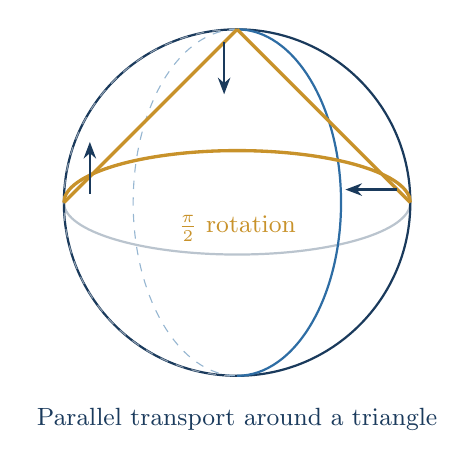
\begin{tikzpicture}[scale=1.1]
% Sphere
\draw[NavyBlue!30, thick] (0,0) ellipse (2cm and 0.6cm);
\draw[NavyBlue, thick] (0,0) circle (2cm);
\draw[NavyBlue!50, dashed] (0,2) arc[start angle=90, end angle=270, radius=2];
% Meridians
\draw[MidBlue, thick] (0,2) arc[start angle=90, end angle=-90, x radius=1.2, y radius=2];
\draw[MidBlue!50, dashed] (0,2) arc[start angle=90, end angle=270, x radius=1.2, y radius=2];
% Triangle on sphere
\draw[Gold, very thick] (0,2) -- (2,0);
\draw[Gold, very thick] (0,2) -- (-2,0);
\draw[Gold, very thick] (2,0) arc[start angle=0, end angle=180, x radius=2, y radius=0.6];
% Parallel transport arrow
\draw[-{Stealth[length=6pt]}, NavyBlue, thick] (0,2) ++ (-0.15,-0.15) -- ++(0,-0.6);
\draw[-{Stealth[length=6pt]}, NavyBlue, thick] (2,0) ++ (-0.15,0.15) -- ++(-0.6,0);
\draw[-{Stealth[length=6pt]}, NavyBlue, thick] (-2,0) ++ (0.3,0.1) -- ++(0,0.6);
\node[font=\small, color=Gold] at (0,-0.3) {$\tfrac{\pi}{2}$ rotation};
\node[font=\small, color=NavyBlue] at (0,-2.5) {Parallel transport around a triangle};
\end{tikzpicture}
\end{center}

\subsection{Step 3: Curvature}

\begin{problem}
\label{prob:curvature}
\begin{enumerate}[label=(\alph*),topsep=2pt]
  \item The \textbf{Riemann curvature tensor} is defined by the failure of parallel transport around an infinitesimal loop:
  $R^k_{\ \ell ij} = \partial_i\Gamma^k_{j\ell}-\partial_j\Gamma^k_{i\ell}+\Gamma^k_{im}\Gamma^m_{j\ell}-\Gamma^k_{jm}\Gamma^m_{i\ell}$.
  On a flat space, $R^k_{\ \ell ij}=0$. Compute one non-zero component of $R^k_{\ \ell ij}$ for $S^2$.
  \item The \textbf{Ricci tensor} $R_{ij} = R^k_{\ ikj}$ (trace of Riemann). The \textbf{Ricci scalar} $R = g^{ij}R_{ij}$ (trace of Ricci). For $S^2$ of radius $r$: $R = 2/r^2$. For flat space: $R=0$. Interpret.
  \item \textbf{Gauss-Bonnet theorem}: for a compact surface $\Sigma$, $\frac{1}{2\pi}\int_\Sigma K\,dA = \chi(\Sigma)$ where $K$ is the Gaussian curvature and $\chi$ is the Euler characteristic. For $S^2$: $K=1/r^2$ everywhere, $\int K\,dA = 4\pi r^2/r^2 = 4\pi$, so $\chi=2$. For a torus: $\int K\,dA=0$, so $\chi=0$. Interpret: the total curvature is a topological invariant.
  \item An alternative formula for curvature: if a circle of geodesic radius $\varepsilon$ has circumference $C(\varepsilon)$, then $K = \lim_{\varepsilon\to 0}\frac{3}{\pi}\frac{2\pi\varepsilon - C(\varepsilon)}{\varepsilon^3}$. Verify for $S^2$ using $C(\varepsilon)=2\pi r\sin(\varepsilon/r)$.
  \item \textbf{Parallel transport around a loop}: the rotation angle of a vector transported around a closed loop $\gamma$ is $\Omega = \int\int_{\text{enclosed}} K\,dA$ (the area integral of the Gaussian curvature). Verify for the puzzle triangle (enclosing $\frac{1}{8}$ of the sphere): $\Omega = K\cdot(\text{area}) = (1)\cdot(\pi/2) = \pi/2 = 90°$.
\end{enumerate}
\end{problem}

\subsection{Step 4: Einstein's field equations}

\begin{problem}
\label{prob:einstein}
The \textbf{Einstein field equations} relate the geometry of spacetime to its matter content:
\[
  G_{\mu\nu} \equiv R_{\mu\nu} - \frac{1}{2}g_{\mu\nu}R = \frac{8\pi G}{c^4}T_{\mu\nu},
\]
where $G_{\mu\nu}$ is the Einstein tensor (encodes curvature), and $T_{\mu\nu}$ is the stress-energy tensor (encodes matter and energy).
\begin{enumerate}[label=(\alph*),topsep=2pt]
  \item The left side is purely geometric (constructed from $g_{\mu\nu}$ and its derivatives). The right side is physical (energy, momentum, pressure of matter). Write in words: what does the equation say?
  \item In vacuum ($T_{\mu\nu}=0$), the equations become $R_{\mu\nu}=0$. This does not mean flat spacetime --- it means Ricci-flat. Show that gravitational waves and black holes are solutions to the vacuum equations.
  \item \textbf{Newtonian limit.} In the weak-field, slow-motion limit, the $00$-component of the Einstein equations reduces to $\nabla^2\Phi=4\pi G\rho$ (Poisson's equation for Newtonian gravity). Identify $\Phi$ as the Newtonian gravitational potential. This shows Newton's law of gravity is the low-curvature, low-velocity limit of GR.
  \item The \textbf{Einstein-Hilbert action} is $S = \frac{c^4}{16\pi G}\int(R-2\Lambda)\sqrt{-g}\,d^4x + S_{\text{matter}}$, where $\Lambda$ is the cosmological constant and $g=\det(g_{\mu\nu})$. Varying with respect to $g^{\mu\nu}$ gives the Einstein field equations. This makes GR the action principle to end all action principles.
  \item \textbf{The cosmological constant.} $\Lambda>0$ gives a repulsive effect at large scales. Einstein introduced it (then regretted it) to make a static universe; it was rediscovered in 1998 when astronomers found the universe's expansion is accelerating. The current measured value is $\Lambda\approx 1.1\times 10^{-52}$ m$^{-2}$. Interpret $\Lambda$ as the energy density of the vacuum. Why is its value the greatest unsolved problem in theoretical physics?
\end{enumerate}
\end{problem}

\begin{problem}
\label{prob:gr_solutions}
\textbf{Exact solutions.}
\begin{enumerate}[label=(\alph*),topsep=2pt]
  \item The \textbf{Schwarzschild metric} (spherically symmetric, vacuum):
  $ds^2 = -\left(1-\frac{r_s}{r}\right)c^2dt^2 + \left(1-\frac{r_s}{r}\right)^{-1}dr^2 + r^2d\Omega^2$,
  where $r_s = 2GM/c^2$ is the Schwarzschild radius. At $r=r_s$, the $g_{tt}$ component vanishes: this is the \textbf{event horizon} of a black hole. Nothing inside can escape. Compute $r_s$ for the Sun ($M_\odot=2\times 10^{30}$ kg) and for the Earth.
  \item A photon follows a null geodesic ($ds^2=0$). For radial motion in the Schwarzschild metric: show that $dr/dt\to 0$ as $r\to r_s$ for a distant observer. Yet for a freely falling observer, crossing the event horizon takes finite proper time. Resolve the apparent paradox.
  \item \textbf{Gravitational redshift.} A clock at radius $r$ in the Schwarzschild metric runs slow by a factor $\sqrt{1-r_s/r}$ relative to a clock at infinity. GPS satellites must account for this (and for special-relativistic time dilation). At an altitude of $20{,}200$ km, compute the net time gain per day.
  \item The \textbf{FLRW metric} describes a homogeneous, isotropic expanding universe: $ds^2 = -c^2dt^2+a(t)^2\left[\frac{dr^2}{1-kr^2}+r^2d\Omega^2\right]$. The Einstein equations with $T_{\mu\nu}$ for a perfect fluid give the \textbf{Friedmann equations} for $a(t)$. For a flat universe ($k=0$) with matter only: show $a(t)\propto t^{2/3}$.
\end{enumerate}
\end{problem}

\section{Part 3 \texorpdfstring{---}{--} Discovery}

\begin{discoverybox}
\textbf{What have we built?}

\textbf{First.} The metric tensor $g_{ij}$ defines geometry on a curved space: distances, angles, areas, volumes. It replaces Euclid's flat-space assumptions with a completely general, coordinate-independent framework.

\textbf{Second.} The Christoffel symbols encode how the basis vectors change across the manifold. Geodesics --- the ``straight lines'' of curved space --- satisfy the geodesic equation $\ddot q^k+\Gamma^k_{ij}\dot q^i\dot q^j=0$.

\textbf{Third.} The Riemann curvature tensor is the fundamental measure of non-flatness. It encodes parallel transport failure around loops. The Ricci tensor and scalar are contractions used in the Einstein equations.

\textbf{Fourth.} The Einstein field equations $G_{\mu\nu}=\frac{8\pi G}{c^4}T_{\mu\nu}$ are the most compact and complete description of gravity. In the Newtonian limit they reduce to Poisson's equation. Their vacuum solutions include gravitational waves and black holes. The cosmological constant controls the large-scale geometry of the universe.

\medskip
\textbf{Journey 4 summary.} Six modules. Vector fields and operators. The integral theorems. Three classical PDEs. Quantum mechanics. Classical mechanics and least action. Curved spaces and general relativity. Every topic used everything that came before.
\end{discoverybox}

\section{Part 4 \texorpdfstring{---}{--} Naming the Ideas}

\begin{namebox}
\textbf{Journey 4 summary table.}
\medskip
\begin{center}
\renewcommand{\arraystretch}{1.5}
\begin{tabular}{l l l}
\toprule
\textbf{Module} & \textbf{Core discovery} & \textbf{Physical content} \\
\midrule
1 & Gradient, divergence, curl & Conservative forces, field lines \\
2 & Integral theorems & Maxwell's equations, conservation laws \\
3 & Laplace, heat, wave PDEs & Electrostatics, diffusion, sound/light \\
4 & Schr\"{o}dinger equation & Quantisation, hydrogen atom, spin \\
5 & Principle of least action & Noether's theorem, Poisson brackets \\
6 & Riemannian geometry & General relativity, black holes, cosmology \\
\bottomrule
\end{tabular}
\end{center}
\end{namebox}

\section{Part 5 \texorpdfstring{---}{--} Deep Problems}

\begin{deepproblem}[Covariant derivative and tensor calculus]
\begin{enumerate}[label=(\alph*)]
  \item The ordinary derivative $\partial_i V^j$ of a vector field is not a tensor (it transforms badly under coordinate changes). Define the \textbf{covariant derivative}: $\nabla_i V^j = \partial_i V^j + \Gamma^j_{ik}V^k$. Show this transforms as a tensor.
  \item The covariant derivative of the metric vanishes: $\nabla_k g_{ij}=0$ (metric compatibility). Show this is equivalent to the definition of $\Gamma^k_{ij}$ via the metric.
  \item The Riemann tensor can be written as the commutator of covariant derivatives: $R^k_{\ \ell ij}V^\ell = (\nabla_i\nabla_j-\nabla_j\nabla_i)V^k$. This shows curvature is exactly the failure of covariant derivatives to commute. Verify for one component on $S^2$.
  \item The \textbf{Bianchi identity}: $\nabla_{[k}R_{\ell m]ij}=0$ (antisymmetrised sum over three indices equals zero). Taking the contracted Bianchi identity gives $\nabla^\mu G_{\mu\nu}=0$. This is the covariant conservation of the Einstein tensor. Show this is consistent with $\nabla^\mu T_{\mu\nu}=0$ (energy-momentum conservation).
\end{enumerate}
\end{deepproblem}

\begin{deepproblem}[Gravitational waves]
In the weak-field limit, write $g_{\mu\nu}=\eta_{\mu\nu}+h_{\mu\nu}$ where $|\,h_{\mu\nu}|\ll 1$.
\begin{enumerate}[label=(\alph*)]
  \item Linearise the Einstein equations in $h_{\mu\nu}$. In the \textbf{transverse-traceless gauge}, show they reduce to the wave equation $\Box\bar h_{\mu\nu}=0$ where $\Box=-\partial_t^2/c^2+\nabla^2$ and $\bar h_{\mu\nu}=h_{\mu\nu}-\frac{1}{2}\eta_{\mu\nu}h$.
  \item A gravitational wave propagating in the $z$-direction takes the form $h_{\mu\nu}=A_{\mu\nu}\cos(kz-\omega t)$ with $\omega=ck$. Only the $h_{xx}=-h_{yy}=h_+$ (plus polarisation) and $h_{xy}=h_{yx}=h_\times$ (cross polarisation) components are non-zero. Describe how a ring of test masses deforms under each polarisation.
  \item LIGO detected the merger of two black holes of masses $36M_\odot$ and $29M_\odot$ in 2015 (GW150914), producing a strain $h\sim 10^{-21}$ at Earth (1.3 billion light-years away). The mirrors moved by $10^{-18}$ m --- one-thousandth the diameter of a proton. Estimate the power radiated at peak: the \textbf{quadrupole formula} gives $P = \frac{G}{5c^5}\langle\dddot{Q}_{ij}\dddot{Q}^{ij}\rangle$ where $Q_{ij}$ is the quadrupole moment. For the merger, $P\approx 3.6\times 10^{49}$ W, greater than the combined luminosity of all stars in the observable universe.
  \item The \textbf{inspiral} phase: two masses in circular orbit lose energy to gravitational radiation, causing the orbit to shrink. The period decreases at a rate predicted by GR. The Hulse-Taylor binary pulsar confirmed this prediction to 0.2\% accuracy before LIGO, earning them the 1993 Nobel Prize.
\end{enumerate}
\end{deepproblem}

\begin{deepproblem}[Topology and global structure]
\begin{enumerate}[label=(\alph*)]
  \item A \textbf{manifold} is a space that looks locally like $\mathbb{R}^n$ but may have a different global structure. The sphere $S^2$, torus $T^2$, and projective plane $\mathbb{RP}^2$ all have the same local geometry (locally flat) but different topology. Describe how the Euler characteristic distinguishes them.
  \item \textbf{Singularity theorems} (Penrose-Hawking): any spacetime satisfying reasonable energy conditions and containing a trapped surface must be geodesically incomplete --- it must have a singularity. This proves that black holes contain singularities and that the Big Bang was a singularity. These theorems use topology (causal structure) rather than an exact solution.
  \item A \textbf{wormhole} (Einstein-Rosen bridge) is a solution to the vacuum Einstein equations connecting two regions of spacetime. Show topologically why a wormhole cannot be traversable without violating energy conditions. (A traversable wormhole would require matter with negative energy density.)
  \item \textbf{The holographic principle} (t'Hooft, Susskind, Maldacena): the information content of a region of spacetime is proportional to the area of its boundary, not its volume. For a black hole, the Bekenstein-Hawking entropy is $S = k_B\frac{A}{4\ell_P^2}$ where $A$ is the event horizon area and $\ell_P = \sqrt{\hbar G/c^3}\approx 1.6\times 10^{-35}$ m is the Planck length. Compute the entropy of a black hole of mass $10M_\odot$. Interpret: information is stored on surfaces, not in volumes.
\end{enumerate}
\end{deepproblem}

\section{Part 6 \texorpdfstring{---}{--} Reflection}

\begin{reflectionbox}
\textbf{Final reflection for Journey 4.}

\begin{enumerate}
  \item \textbf{On the nature of gravity.} Newton's gravity is a force acting instantaneously across empty space. Einstein's gravity is the geometry of spacetime, with no force and no action at a distance. Both make the same predictions in the weak-field, slow-motion limit. Write a paragraph: what does it mean for two theories to be empirically equivalent but conceptually completely different? Which is ``right''?

  \item \textbf{On the unreasonable effectiveness of mathematics.} Riemannian geometry was developed in 1854 as pure mathematics with no physical application. Einstein applied it to physics in 1915. The mathematics came first. Write about one other case from this curriculum where mathematics developed independently of physics turned out to be exactly what physics needed.

  \item \textbf{On the cosmological constant.} The vacuum energy predicted by quantum field theory is $10^{120}$ times larger than the observed cosmological constant. This is the largest discrepancy between theory and observation in the history of science. Write a sentence on what this suggests about our understanding of physics.

  \item \textbf{Looking ahead.} Journey~5 studies probability and uncertainty --- not quantum uncertainty, but classical probability theory, statistics, and information theory. How does the probabilistic language of Journey~5 connect to quantum mechanics (Journey~4 Module~4)? Is quantum probability the same as classical probability with a different rule?
\end{enumerate}
\end{reflectionbox}

\vspace{0.8cm}
\begin{namebox}
\textbf{What Journey 4 built --- and where it feeds.}

\medskip
Journey~4 built the mathematics of physical space and fields. The vector calculus operators (Module~1--2) are the language of all continuum physics. The three classical PDEs (Module~3) govern heat, electrostatics, and wave propagation --- and they appear again in quantum mechanics (Module~4) and general relativity (Module~6). The principle of least action (Module~5) underlies every fundamental physical theory. Curved spaces (Module~6) are the arena for general relativity and the geometry of the entire universe.

\medskip
Journey~5 (Uncertainty) builds probability theory, statistics, and information theory --- the mathematics of ignorance and knowledge. It feeds into quantum mechanics (where probability is intrinsic), statistical mechanics (where probability explains thermodynamics), and data science.

Journey~6 (Transformation) builds Fourier analysis, spectral methods, and signal processing --- the mathematics of frequency. It is the spectral theory of the differentiation operator applied in full, unifying PDEs, quantum mechanics, and communications.

Journey~7 (Abstraction) unifies everything through groups, rings, and categories.

\medskip
You are now more than halfway through the curriculum. The mathematics and physics you know already would be remarkable for a professional scientist. The questions that remain are the hardest ones.
\end{namebox}

\vspace{1cm}
\begin{center}
{\color{Gold}\rule{0.6\linewidth}{1.2pt}}\\[8pt]
{\large\bfseries\color{NavyBlue}End of Journey 4: Fields and Space}\\[6pt]
{\normalsize\color{DarkGrey}\itshape Six modules. Vector fields, integral theorems, classical PDEs,\\
quantum mechanics, the action principle, and general relativity.}\\[10pt]
{\color{Gold}\rule{0.6\linewidth}{1.2pt}}\\[10pt]
{\small\color{DarkGrey}Continue to: \textbf{Journey 5 --- Uncertainty}}\\[4pt]
{\small\color{DarkGrey}\itshape ``The most beautiful thing we can experience is the mysterious.\\
It is the source of all true art and all science.''\\
\upshape --- Albert Einstein}
\end{center}

\end{document}